% Template for ICASSP-2026 paper; to be used with:
%          spconf.sty  - ICASSP/ICIP LaTeX style file, and
%          IEEEbib.bst - IEEE bibliography style file.
% --------------------------------------------------------------------------
\documentclass{article}
\usepackage{spconf,amsmath,graphicx,hyperref}
\usepackage{comment}
%\usepackage[preprint]{aistats2026}
\usepackage{subcaption}
\usepackage{graphicx}
\usepackage{xparse}
\usepackage{tikz}
\usepackage{multirow}
\usetikzlibrary{spath3,arrows.meta}
% Example definitions.
% --------------------
\def\x{{\mathbf x}}
\def\L{{\cal L}}

% Title.
% ------
\title{Lighting Transfer for Nighttime Image Enhancement with Weak Daytime References}
%
% Single address.
% ---------------
\name{Junda Wang \and Rundong Cao \and Jiazhong Yu \and Linsu Shi \and Ziwei Liu \and Sheng Cao \and Ton Lin\thanks{Thanks to XYZ agency for funding.}}
\address{Author Affiliation(s)}
%
% For example:
% ------------
%\address{School\\
%	Department\\
%	Address}
%
% Two addresses (uncomment and modify for two-address case).
% ----------------------------------------------------------
%\twoauthors
%  {A. Author-one, B. Author-two\sthanks{Thanks to XYZ agency for funding.}}
%	{School A-B\\
%	Department A-B\\
%	Address A-B}
%  {C. Author-three, D. Author-four\sthanks{The fourth author performed the work
%	while at ...}}
%	{School C-D\\
%	Department C-D\\
%	Address C-D}
%
\begin{document}
%\ninept
%
\maketitle
%
\begin{abstract}
Low-Light Image Enhancement (LLIE) is a crucial computer vision task that aims to improve visibility under weakly illuminated conditions. In conventional supervised settings, short/long exposure RAW images are captured by the same camera at daytime to obtain low/normal light pairs. Models trained on these “bogus” datasets often struggle with nighttime images under different illumination conditions. This paper introduces the Adaptive Lighting Transfer Network (ALTNet), a domain-tailored framework for Nighttime Image Enhancement (NIE). The illumination characteristics of the daytime references are transferred to the nighttime images for illumination enhancement. Our method is flexible enough to allow the referenced daytime image to play a role both in the training and testing phases, and to permit different objects or humans occurring in the scene without the need of exact pixel alignment. Extensive experiments on various benchmark datasets demonstrate the effectiveness of the proposed ALTNet. 
\end{abstract}
%
\begin{keywords}
Low-light transfer, WCT
\end{keywords}
%
\section{Introduction}
\label{sec:intro}




Low-Light Image Enhancement (LLIE) aims to improve the brightness and visibility of such images. The ideal outcome is to produce a result that appears as if it was captured under normal lighting conditions, while preserving the original content (\cite{surveyli}). LLIE has been applied in various fields, including nighttime surveillance, autonomous driving, and photo editing (\cite{surveykbs}).




Traditional methods for the LLIE problem can be categorized primarily into histogram equalization-based approaches (\cite{he}) and Retinex-based approaches (\cite{retinex}). Histogram equalization-based methods aim to adjust the original pixel distribution. On the other hand, Retinex-based methods are founded on the Retinex theory, which posits that an image can be decomposed into an illumination component and a reflection component. Conventional methods often struggle with diverse lighting conditions and exhibit limited performance. 


Nowadays, deep learning-based approaches have recently emerged as the dominant paradigm in LLIE, owing to their powerful ability to model complex non-linear relationships. \textcite{retinex} proposed the first Retinex-based deep networks that adaptively decompose the input images and used another Enhance-Net to adjust the illumination. In addition, several advanced models in other domains have been migrated to LLIE for superior performance. \textcite{retinexformer} designed an Illumination-Guided Transformer (IGT) that captures the non-local relationship of regions with different lighting conditions. \textcite{lldiff} presented a conditional diffusion model to produce satisfactory results with a powerful generation ability. More recently, \textcite{hvicidnet} proposed a new HVI color space to decouple brightness from chrominance and a two-branch CIDNet with cross-attention, achieving state-of-the-art results on ten paired benchmarks. \textcite{retidiff} combined the Retinex prior with a latent diffusion model, where a Retinex-guided transformer uses the generated reflectance and illumination priors to restore degraded images with strong generative capacity. Beyond paired supervised learning, \textcite{zerodce++} took a zero-reference unsupervised route, training a lightweight curve-estimation network with non-reference losses (spatial consistency, exposure control, color constancy and illumination smoothness), enabling real-time enhancement without any paired or unpaired data.



However, perfectly matched image pairs are necessary for supervised learning methods, which are often impractical to obtain in real-world scenarios. Typically, low-light images in existing datasets are captured by adjusting camera exposure and ISO settings, as seen in LOLv1 (\cite{retinex}), LOLv2 (\cite{lolv2}) and SID (\cite{SID}). Such datasets fail to adequately represent the diverse degradation patterns present in authentic nighttime images or those captured under genuinely poor illumination conditions. In contrast, unsupervised learning methods depend only on nighttime images without requiring reference pairs. Nevertheless, the absence of reference images during training results in inferior performance compared to supervised approaches. More importantly, both supervised and unsupervised methods essentially learn an end-to-end mapping from low-light inputs to ideal outputs, akin to ``seeing the light only from the dark''. This formulation significantly increases the difficulty of the LLIE problem. 



To address these issues, we first design a new formulation of collecting weakly paired dataset. The daytime and nighttime image pairs are captured at the same scene at different time and illumination conditions. Besides, moving objects (\textit{e.g.}, pedestrians, cars and bycycles) are allowed to occur or vanish and there is no need to align them. Such images pairs are practical to be collected and can reflect true illumination conditions, which is helpful for the Nighttime Image Enhancement (NIE). In addition, we propose a novel NIE paradigm, termed as lighting transfer, which strives to transfer the lighting condition of daytime references to nighttime images in both the training and inference phases, as shown in Fig.\ref{fig:heading}. 



Our main contributions are as follows:

\begin{itemize}
    \item We collect a weakly paired dataset, called DNP (Daytime-Nighttime image Pairs). Data pairs record similar scenes and allow for variations in the moving objects (e.g., vehicles and pedestrians). In addition, DNP is able to represent the real lighting conditions change, such as the sunshine and streetlamps, which is conducive to application in real scenarios.


    
    \item We introduce a novel Nighttime Image Enhancement(NIE) paradigm, \textit{i.e.}, lighting transfer, for the weakly supervised setting. The learning goal is to transfer the lighting condition from daytime images with similar scenes, which makes the task easier since there are illumination references both in the training phase and the inference phase.

opted in the style transfer domain, ALTNet  decrease the perplexity of the model and helping preseving the content affinity.

    \item We propose a simple network named the Adaptive Lighting Transfer Network (ALTNet). The model concatenates both deep features and input images into the transfer module, with the final output obtained by directly extracting the three RGB channels from the transfer result. This design enables the lighting transfer to be learned in a flexible and adaptive manner. Moreover, unlike typical style transfer methods that rely on encoder-decoder architectures, ALTNet reduces model complexity and better preserves content consistency and structural fidelity.

\end{itemize}

\section{RELATED WORKS}
\paragraph{Unpaired NIE.} NIE can be mainly divided into three classes: supervised learning, unsupervised learning and unpaired learning. Supervised learning-based methods need perfectly matched ground truth as pixel-level supervisory signals, whereas unsupervised learning-based methods only need nighttime input and highly depend on handcrafted priors. Unlike supervised and unsupervised learning, unpaired LLIE is trained on two independent sets of low-light and normal-light images. It combines the advantages to achieve an excellent result while reducing the requirement for strict pairing. \textcite{enlightengan} used a global-local discriminator to examine the enhanced results. \textcite{cycleretinex} incorporated the Retinex theory into the generative adversarial network. \textcite{invertibleLLIE} utilzed the invertible network to enhance low-light images and degrade the normal-light images inversely. \textcite{lightendiffusionjiang2024} presented a content decomposition network to obtain content-rich reflectance maps and content-free illumination maps before the diffusion model.


\paragraph{Style Transfer.}
Style transfer aims to change the style of the image without affecting the content. \textcite{gatys2016image} utilized the convolution layers in VGG to extract the high level representation of images and matched the correlation of deep features. Following the encoder-decoder architecture, many feature transformation modules have been proposed. \textcite{adain} matched the mean and variance of deep features. \textcite{li2017universal} employed the Whitening and Coloring Transform (WCT) to match the inter-channel correlation. \textcite{wct2} leveraged a wavelet corrected transfer to enhances photorealism. \textcite{capvst} adopted the reversible residual network to keep the content affinity.

\section{DATASET PREPARATION} \label{sec:dataset}

\begin{figure}[htbp]
\setlength{\tabcolsep}{1pt} % 极小的列间距
\vspace{-0.15in}
%\centerline{\fbox{This figure intentionally left non-blan}}
\centering
\begin{tabular}{ccc}
    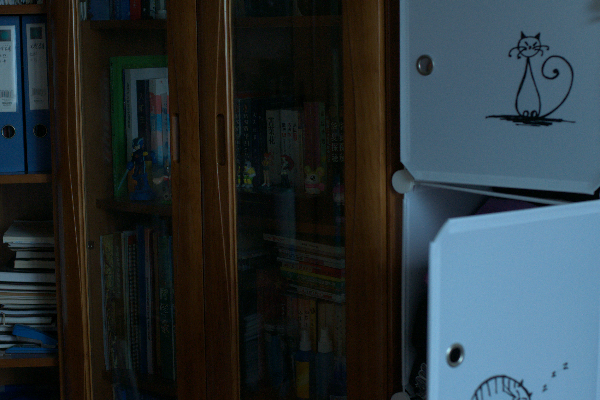
\includegraphics[width = 0.32\linewidth]{figures/multiply/1_low.png} &
    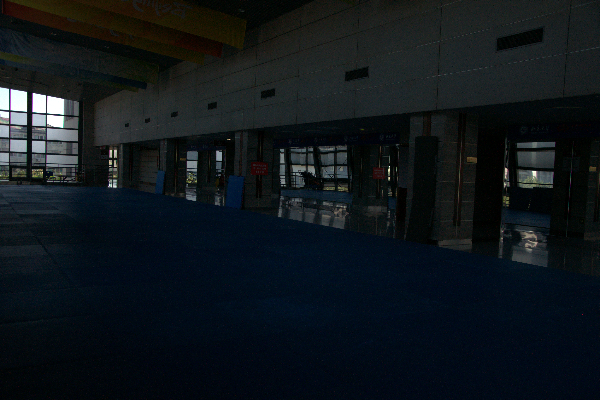
\includegraphics[width = 0.32\linewidth]{figures/multiply/780_low.png} & 
    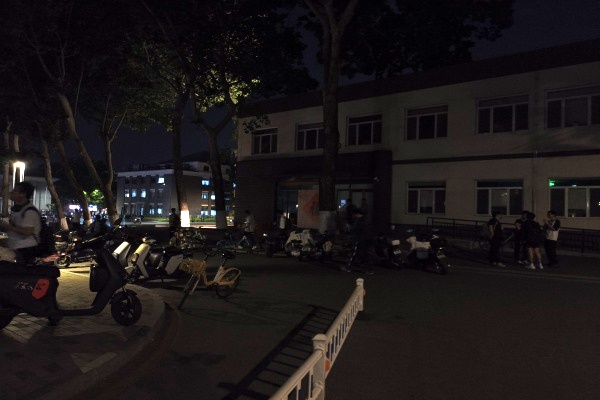
\includegraphics[width = 0.32\linewidth]{figures/multiply/22 (12) low.jpg}  \\
    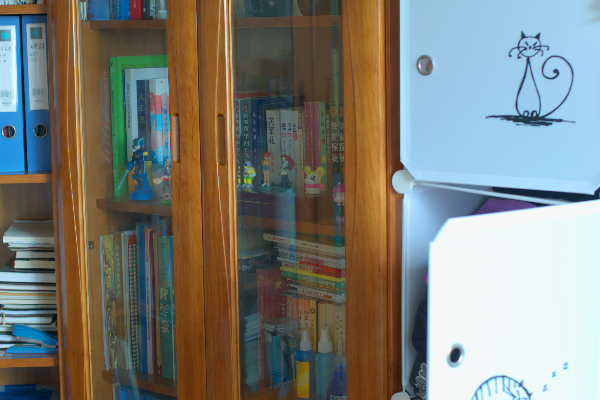
\includegraphics[width = 0.32\linewidth]{figures/heading/1.png} &
    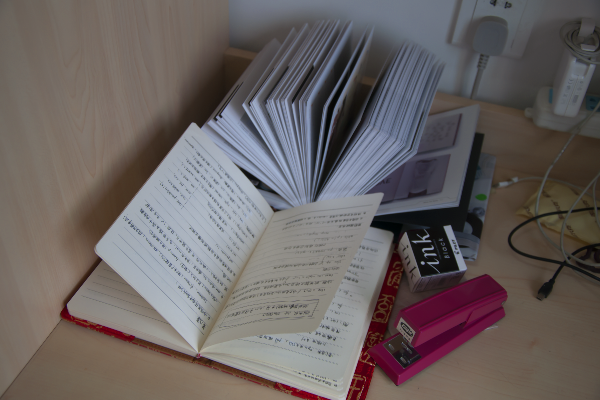
\includegraphics[width = 0.32\linewidth]{figures/heading/547.png} & 
    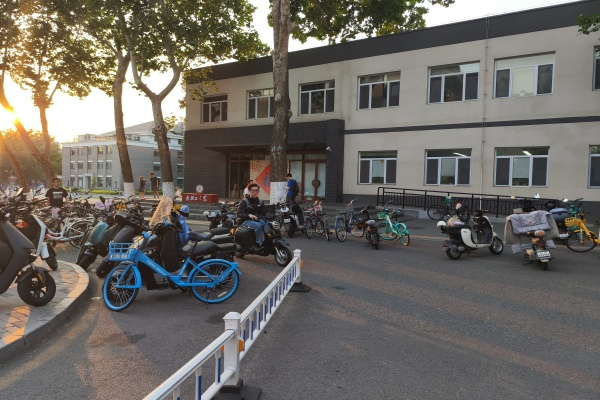
\includegraphics[width = 0.32\linewidth]{figures/transform/22 (12).jpg}  \\
    
    
     
     Paired & Unpaired & Weakly paired\\
     
\end{tabular}
%\vspace{-in}
\caption{The comparison of different dataset: perfectly paired, unpaired and the proposed weakly paired dataset. The low-light images are multiplied by 3 for better visual effect.}\label{fig:dataset}
\end{figure}

It is impossible to capture the nighttime and daytime images simultaneously. For some prevalent paired dataset, such as LOLv1 and LOLv2, the corresponding low-light images are captured by changing the camera sensor exposure and ISO settings. They can not reflect the various degradation problems in the night environment, like high noise level and complex light condition. Furthermore, the low-light and normal-light pairs need to be strictly aligned at the pixel level, which makes collecting more difficult. The unpaired dataset, where the low-light images and normal-light images are independent, can not provide precise light information, increasing the learning complexity.


To cope with the above problems, we introduce a new weakly paired dataset, whose image pairs are scene-consistent but semantically variant. Specifically, the image pairs are taken in the same scene during the day and at night, respectively. Thus, the image pairs are able to reflect the real degradation problem. Besides, dynamic objects (e.g., vehicles, pedestrians) may appear, disappear, or change positions at different times. Therefore, the image pairs have variant semantics. It is impossible and unnecessary to perfectly match them at the pixel level, which has greatly reduced the difficulty of collection. In short, we refer to this readily available dataset as the DNP (Daytime-Nighttime image Pairs). We used a mobile phone camera with default parameters to collect 344 pairs of images (317 for training and 27 for testing) from different scenes on an anonymous campus. Examples of DNP and the difference with other datasets are shown in Fig.\ref{fig:dataset}.


\section{METHODOLOGY}


\subsection{Motivation and a Toy Experiment}\label{sec:motivation}





In the weakly paired dataset, the nighttime images contain the content while daytime images have the desired lighting conditions in similar scenes. Intuitively, the lighting condition can seem as a kind of image style. Consequently, the NIE task belongs to the photorealistic style transfer problem. There are various style transfer modules, such as InstanceNorm (\cite{adain}) and WCT (\cite{li2017universal}). Naively, the transform module can be applied directly in the image itself. Nighttime images will be re-stretched to conform to the distribution of daytime images. To validate this assumption, we conduct a toy experiment using the WCT module solely on the LOLv1 dataset. This experiment aimed to transfer the illumination condition from matched normal-light to low-light images. Since the transformation relies on global statistics rather than pixel-level value, the image pairs do not need to be pixel-aligned. This allows us to use randomly cropped portions (denoted as $\alpha$) of the normal-light images, providing varying amounts of lighting information. As shown in Fig.~\ref{fig:toytest}, even a small crop of a normal-light image can produce an enhanced result with satisfactory illumination. Moreover, as the ratio increases, the stylized images are closer to the target images. This toy experiment inspired us to develop the ALTNet which is described in the following subsection. 






\subsection{Adaptive Lighting Transfer Network}



Motivated by the effectiveness of the statistics provided by the daytime references, we proposed an Adaptive Light Transfer Network (ALTNet). The architecture diagram of the proposed ALTNet is illustrated in Fig.~\ref{fig:structure}.

Firstly, a simple feature extraction module that contains several convolution layers is utilized to obtain deep feature as the usual encode layer. Rather than applying the transformation only in the feature space, the input image $I\in\mathbb{R}^{3\times H\times W}$ is concatenated at the end of the feature to form an augmented feature $Z\in\mathbb{R}^{C\times H\times W}$, which can expressed as follows:
\begin{equation}
    %\hat{Z}_{night} &=  \text{concat}(F_{\theta}(I_{night}), I_{night})\\
    %\hat{Z}_{day} &=  \text{concat}(F_{\theta}(I_{day}), I_{day})\\
    \begin{split}
    Z_{night} &=  {concat}(F_{\theta}(I_{night}), I_{night}),\\
    Z_{day} &=  {concat}(F_{\theta}(I_{day}), I_{day}).
     \end{split}
\end{equation}
$I_{day}$ and $I_{night}$ are the weakly paired daytime and nighttime images, and $F_\theta$ represents the encoder. 

Subsequently, the lighting transfer module migrates the lighting condition of $Z_{day}$ to $Z_{night}$, generating $Z_{transfer}$. The distinction is that this method does not require a decoder to obtain stylized images. The three channels at the tail of $Z_{transfer}$ can naturally be regarded as stylized images. We only need to separate these three channels to obtain the final result $I_{transfer}$, which can be shown as:
\begin{equation}
    \begin{split}
    Z_{transfer} &=  {LT}(Z_{night},  Z_{day}),\\
    I_{transfer} &= Z_{transfer}[-3:,:,:].
    \end{split}
\end{equation}
$LT$ is the alternative lighting transfer module, and $[-3:,:,:]$ represents the slice operation to extract the last three channels. Without the encoder-decoder architecture, the risk of introducing artifacts and content distortion is naturally reduced.

Theoretically, we can choose any transformation module in the lighting transfer part. If we only match the standard deviation of each channel as AdaIN (\cite{adain}) does, there will be no connection between different channels. Then the final result will be the same as directly applying the transfer module to the image. To ensure that the different channels of $Z$ can influence each other, we adopt the WCT (\cite{capvst}), to match the inter-correlation. Since the features extracted by the encoder can be updated when minimizing the loss item, the proposed lighting transfer mechanism is endowed with flexibility and adaptability.

WCT is composed of two steps: whitening and coloring transform. Its purpose is to make the content have the same inter-channel covariance as the style. Firstly, we perform the Choleskey decomposition on the covariance matrix, whose computational cost is much lower that that of SVD. $Z_{night}$ and $Z_{day}$ are regarded as matrices of shape $C$ by $H\times W$ and the process can be expressed as:
\begin{equation}
    \begin{split}
    \bm{\Sigma}_{Z_{night}} =&(Z_{night}-\mu(Z_{night}))(Z_{night}-\mu(Z_{night}))^T\\
    =&S_{night}S^T_{night},\\
    \bm{\Sigma}_{Z_{day}} =&(Z_{day}-\mu(Z_{day}))(Z_{day}-\mu(Z_{day}))^T\\
    =&S_{day}S^T_{day},\\
        %S_{day}S^T_{day} =&  (Z_{day}-\mu(Z_{day}))(Z_{day}-\mu(Z_{day}))^T,\\
        %S_{night}S^T_{night} =&  (Z_{night}-\mu(Z_{night}))(Z_{night}-\mu(Z_{night}))^T,
    \end{split}
\end{equation}
where $S\in \mathbb{R}^{C\times C}$ is the lower triangular matrix obtained by performing the Choleskey decomposition on the covariance matrix $\bm{\Sigma}$.



Subsequently, the inverse of $S_{night}$ is used to remove the correlation of $Z_{night}$, known as whitening. This is followed by a coloring operation through multiplication with $S_{day}$, which can be formulated as:
\begin{equation}
    \begin{split}
        %S_{day}S^T_{day} =&  (Z_{day}-\mu(Z_{day}))(Z_{day}-\mu(Z_{day}))^T,\\
        %S_{night}S^T_{night} =&  (Z_{night}-\mu(Z_{night}))(Z_{night}-\mu(Z_{night}))^T,\\
        Z_{transfer} = & LT(Z_{night},Z_{day})\\
        =& S_{day}S^{-1}_{night}(Z_{night}-\mu(Z_{night}))\\
        &+\mu(Z_{day}).
    \end{split}
\end{equation}

Now, $Z_{transfer}$ shares the inter-channel correlation of $Z_{day}$, thus achieving the desired lighting transfer:
\begin{equation}
    \begin{split}
        \bm{\Sigma}_{Z_{transfer}} = &(Z_{transfer}-\mu(Z_{trasnfer}))\\
        &(Z_{transfer}-\mu(Z_{transfer}))^T\\
        =&S_{day}S^{-1}_{night}(Z_{night}-\mu(Z_{night}))\\
        &(Z_{night}-\mu(Z_{night}))^TS^{-T}_{night}S^{T}_{day}\\
        =&S_{day}S^T_{day}\\
        =&\bm{\Sigma}_{Z_{day}}.
    \end{split}
\end{equation}





\subsection{Loss}
In the weakly paired dataset, real daytime images have scenes similar to those of night images, but the specific objects can be different. Therefore, there is no pixel-level ground truth as in supervised learning. As discussed above, the NIE task can be seen as a kind of style transfer problem. The widely used style loss $L_{style}$ makes $I_{transfer}$ have a lighting condition more similar to $I_{day}$, which is formulated as follows: 
\begin{equation}
\begin{split}
    L_{style} = \sum_{i=1}^l \|\mu(\phi_i(I_{\text{transfer}})) - \mu(\phi_i(I_{\text{day}}))\| \\
    + \sum_{i=1}^l \|\sigma(\phi_i(I_{\text{transfer}})) - \sigma(\phi_i(I_{\text{day}}))\|,
\end{split}
\end{equation}
where $\phi_i$ denotes the $i_{th}$ layer of
the VGG-19 network (from ReLu1$\_$1 to ReLu4$\_$1). $\mu$
and $\sigma$ denote the mean and variance, respectively.


In the lighting transfer stage, the final enhanced image $I_{transfer}$ is calculated as a weighted linear transformation of $Z_{night}$ within the WCT framework. The adaptability afforded by this blending operation comes at the cost of a risk of blurring. Hence, the usual reconstruction loss is adopted to reduce blurring and improve training stability. Specifically, we cyclically transfer the lighting condition of $I_{night}$ to $I_{trasnfer}$ to obtain reconstructed nighttime images $\widetilde{I}_{night}$. The reconstruction loss can be formulated as follows:
\begin{equation}
    L_{rec} = ||I_{night}-\widetilde{I}_{night}||_1.
\end{equation}

The total loss is a weighted sum of two specific losses:
\begin{equation}
    L = \lambda_{style}L_{style} + \lambda_{rec}L_{rec}.
\end{equation}



\subsection{Inference with Weak References}




In the proposed ALTNet, the daytime references are input into the networks in both the training and the inference phases. Although a weakly paired reference image is required, it is not difficult to obtain and allows for different lighting conditions, different moving objects, and does not require strict pixel alignment. The toy example shown in Sec.\ref{sec:motivation} has proved the great efficiency brought about by the daytime images. For some specific application scenarios, ALTNet will demonstrate significant advantages over other existing methods that ignore daytime references. For instance, in a fixed point night surveillance scenario, it is easy to record the daytime images of the surrounding environment. We can choose one as a reference to enhance the night images. Additionally, ALTNet uses relatively few parameters, which is very helpful for application deployment on such edge devices. Moreover, the ALTNet does not learn how to directly enhance the input image, but rather how to transfer the lighting conditions of the reference image to the night image. As long as there is a suitable reference image, the risk of insufficient enhancement or color shift is greatly reduced, which significantly enhances generalizability.



\section{EXPERIMENTS}


In the experiments, we first compare the performance of different methods on the DNP dataset. Then, we evaluated the generalization ability of the proposed ALTNet with pretrained weights on other public dataset. Among them, LOLv1 \cite{Retinexnet}), LOLv2-syn and LOLv2-real (\cite{lolv2}) are perfectly paired, while Bdd100k (\cite{bdd100k}), ExDark (\cite{exdark}) and LLVIP (\cite{llvip}) contain only nighttime images. Finally, ablative experiments are conducted to check the effect of each component.
% public results  not fair experiment (ratio)

\subsection{Implementation Details}
We implement ALTNet by PyTorch. The encoder networks contain 4 consecutive convolution layers and the number of ${Z}$ channels is 32. The model is trained with the Adam optimizer, with an initial learning rate of $10^{-4}$ and a decay factor of $5\times10^{-5}$. In the training process, the images are resized to $512\times 512$ and patches at the size of $256\times 256$ are randomly cropped as input. The batch size is 8 and we train ALTNet for 50 epochs, costing about 1.2 hours on a single Nvidia 4090 GPU. The objective is to minimize the style loss $l_{style}$ between the enhanced images and the daytime images, as well as the reconstruction loss $L_{rec}$ between the reconstructed images and the nighttime images. The loss weights $\lambda_{style}$ and $\lambda_{rec}$ are set to 1 and 10, respectively.

\subsection{Nighttime Image Enhancement}

%For other methods used for comparison, both the optimal pretraining weights and the weights obtained through retraining on the DNP dataset are both evaluated.
First, we conduct experiments on our DNP dataset. Existing LLIE methods are divided into three main catogories: supervised learning, unsupervised learning, and unpaired learning. 
RetinexFormer (\cite{retinexformer}) is based on supervised learning. ZeroDCE (\cite{zero-dceplus}), RUAS (\cite{RUAS}) and SCI (\cite{sci}) are unsupervised learning-based. Cycle-Retinex (\cite{cycleretinex}), LightenDiffusion (\cite{lightendiffusionjiang2024}) and SelfEnNet (\cite{selfennet}) are unpaired learning-based. Besides, two style transfer methods, \textit{i.e.}, AdaIN (\cite{adain}) and CAP-VST (\cite{capvst}), participate in the comparison. Among them, unpaired learning-based methods and style transfer methods are the most relevant to the proposed lighting transfer method, since they both use imperfectly paired images for training. Since there is no ground truth in the DNP dataset, we adopt several no-reference metric: NIQE (\cite{niqe}), PI (\cite{pi}), and MUSIQ (\cite{musiq}). NIQE is a completely blind metric that measures the distance between natural image statistics and those of the test image. PI is a sharpness metric combining a set of hand-crafted metrics. MUSIQ is a transformer-based method that processes images at multiple scales.
\subsubsection{Quantitative Results}



\begin{table}[htbp]
\fontsize{8}{8}\selectfont
\caption{Performance metrics on the DNP dataset. The methods with $*$ employ the optimal pretrained weights as the origin papers. Otherwise, they are trained from scratch on the DNP dataset. \textbf{Bold} indicates the best results and \underline{underline} indicates the second best.} \label{tab:dnp}
\centering
\begin{tabular}{l|c|ccc}
\textbf{Methods} & \textbf{Size(M)} & \textbf{NIQE}$\downarrow$ & \textbf{PI}$\downarrow$ & \textbf{MUSIQ}$\uparrow$ \\
\hline
\multicolumn{5}{c}{\textbf{Supervised Learning}} \\
\hline
RetinexFormer & \multirow{2}{*}{1.61}& 6.72 & 6.98 & 16.66 \\
RetinexFormer* & & 3.07 & 2.27 & 58.10  \\
\hline
\multicolumn{5}{c}{\textbf{Unsupervised Learning}} \\
\hline
ZeroDCE & \multirow{2}{*}{0.079} & 3.29 & 2.32 & 59.55 \\
ZeroDCE* & & 3.15 & 2.19 & 59.89 \\
RUAS & \multirow{2}{*}{0.003} & 5.49 & 4.04 & 51.40 \\
RUAS* & & 5.30 & 3.89 & 50.68 \\
SCI & \multirow{2}{*}{0.0003} & 3.72 & 3.02 & 48.87 \\
SCI* & & 3.32 & 2.25 & 59.77 \\
\hline
\multicolumn{5}{c}{\textbf{Unpaired Learning}} \\
\hline
Cycle-Retinex & \multirow{2}{*}{6.78} & 3.23 & 2.22 & \textbf{62.81} \\
Cycle-Retinex* & & \underline{2.99} &\underline{2.12} & \underline{62.52} \\
LightenDiffusion* & 27.83 & 3.45 & 2.57 & 56.81 \\
SelfEnNET & \multirow{2}{*}{0.17} & 3.39 & 2.86 & 57.47 \\
SelfEnNET* & & 3.33 & 2.94 & 54.76 \\
\hline
\multicolumn{5}{c}{\textbf{Transfer Learning}} \\
\hline
AdaIN & \multirow{2}{*}{23.59} & 3.45 & 2.46 & 59.19 \\
AdaIN* & & 3.23 & 2.46 & 56.18 \\
CAP-VST & \multirow{2}{*}{4.09} & 3.12 & 2.24 & 60.81 \\
CAP-VST* & & 3.43 & 2.45 & 58.16 \\
\hline
ALTNet(ours) & 0.09 & \textbf{2.98} & \textbf{2.04} & 61.61 \\
\hline
\end{tabular}
\end{table}

\begin{table*}[htbp]
\centering
\small
\caption{Generalization performance metrics on the LOL dataset. The methods with $*$ employ the optimal pretrained weights as the origin papers. Otherwise, they are trained from scratch on the DNP dataset. \textbf{Bold} indicates the best results and \underline{underline} indicates the second best. Note that RetinexFormer$*$ is excluded from comparison as it is directly supervised on the LOL dataset.}
\label{tab:generation}
\begin{tabular}{l|c|cc|cc|cc}
\hline
\multirow{2}{*}{\textbf{Methods}}  &\multirow{2}{*}{\textbf{Size(M)}}& \multicolumn{2}{c|}{\textbf{LOL-v1}} & \multicolumn{2}{c|}{\textbf{LOL-v2-real}} & \multicolumn{2}{c}{\textbf{LOL-v2-syn}} \\
\cline{3-8}
 && \textbf{PSNR$\uparrow$} & \textbf{SSIM$\uparrow$} & \textbf{PSNR$\uparrow$} & \textbf{SSIM$\uparrow$} & \textbf{PSNR$\uparrow$} & \textbf{SSIM$\uparrow$} \\
\hline

\multicolumn{8}{c}{\textbf{Supervised Learning}} \\
\hline
RetinexFormer&\multirow{2}{*}{1.61}& 13.434 & 0.285 & 12.058 & 0.246 & 11.366 & 0.298 \\
RetinexFormer* & &25.154 & 0.840 & 28.977 & 0.894 & 16.190 & 0.664 \\
\hline

\multicolumn{8}{c}{\textbf{Unsupervised Learning}} \\
\hline
ZeroDCE & \multirow{2}{*}{0.079}&15.597 & 0.482 & 13.744 & 0.461 & 14.709 & 0.643 \\
ZeroDCE* && 14.861 & 0.586 & 18.059 & 0.604 & 17.756 & 0.724 \\
RUAS & \multirow{2}{*}{0.003}&15.290 & 0.570 & 16.097 & 0.528 & 13.772 & 0.582 \\
RUAS*  && 16.405 & 0.581 & 15.326 & 0.517 & 13.404 & 0.577 \\
SCI & \multirow{2}{*}{0.0003}&9.890 & 0.109 & 12.119 & 0.179 & 12.881 & 0.201 \\
SCI*  & &13.806 & 0.532 & 17.253 & 0.574 & 16.695 & 0.654 \\
\hline

\multicolumn{8}{c}{\textbf{Unpaired Learning}} \\
\hline
Cycle-Retinex& \multirow{2}{*}{6.78}& 16.813 & 0.741 & 19.632 & 0.753 & 18.478 & 0.791 \\
Cycle-Retinex* && 18.351 & 0.756 & 19.975 & 0.757 & 18.973 & 0.799 \\
LightenDiffusion* &27.83& 20.447 & 0.760 & 22.874 & 0.800 & \underline{21.559} & \textbf{0.852} \\
SelfEnNet & \multirow{2}{*}{0.17}&16.542 & 0.589 & 18.920 & 0.645 & 18.051 & 0.696 \\
SelfEnNet*  && 16.077 & 0.603 & 20.404 & 0.672 & 16.275 & 0.665 \\
\hline

\multicolumn{8}{c}{\textbf{Transfer Learning}} \\
\hline
AdaIN & \multirow{2}{*}{23.59}&14.201 & 0.477 & 16.865 & 0.498 & 14.730 & 0.550 \\
AdaIN* &  &16.038 & 0.556 & 19.161 & 0.560 & 17.111 & 0.613 \\
CAP-VSTNet&\multirow{2}{*}{4.09}& 21.476 & 0.755 & 23.650 & 0.792 & 18.510 & 0.726 \\
CAP-VSTNet*  & &\underline{23.018} & \textbf{0.811} & \underline{25.115} & \textbf{0.840} & 21.049 & 0.825 \\
\hline
ALTNet(ours)& 0.09 & \textbf{24.734} & \underline{0.785} & \textbf{26.693} & \underline{0.816} & \textbf{22.921} & \underline{0.825} \\
\hline
\end{tabular}
\end{table*}



We quantitatively compare the proposed ALTNet with other SOTA LLIE methods and style transfer methods, as shown in Tab.~\ref{tab:dnp}. Our method outperforms other methods in NIQE and PI, and has a promising result in MUSIQ. Except for the unsupervised learning-based methods, the ALTNet has the smallest number of parameters. The results demonstrate the efficiency of the proposed ALTNet, which contains only several convolution layers. Compared with directly using the optimal pre-training weights, other LLIE methods perform worse after retraining on the DNP dataset. A reason is that in their original training process, datasets containing more images and with better image quality were used. The true daytime and nighttime images of the DNP dataset make it more difficult to learn valuable information. Conversely, the proposed ALTNet learns to transfer the lighting condition of daytime images to nighttime images, rather than learning a brutal mapping to enhance the nighttime images. Therefore, the proposed ALTNet outperforms other methods on the weakly paired dataset.



\subsubsection{Qualitative Results}

Fig.~\ref{fig:DNPresult} shows several test results of different methods on the DNP dataset. SCI has the minimal parameter size, which leads to insufficient enhancement. Unpaired learning-based methods, Cycle-Retinex and SelfEnNet, have severe artifacts around the building and on the road surface. Visually, transfer learning-based methods generate the results with most similar lighting conditions with daytime references. However, AdaIN is not able to cope with photorealistic style transfer, whose results have a distinct blocking effect. CAP-VST adopts a reversible network and various loss functions to keep content affinity, but still causes overexposure and blurring. The proposed ALTNet abandons the widely used encoder-decoder structure, which naturally reduces the risk of generating artifacts and greatly lowers the parameter requirements. In summary, the proposed ALTNet is a simple but efficient lighting transfer method.


\subsection{Generalization Evaluation}
\



In this part, we demonstrate the superior generalizability of the proposed ALTNet on other public dataset without extra training. LoLv1, LOLv2-real, LOLv2-syn are paired dataset and we directly use the matched normal-light images as references to input into the transfer learning-based methods (including the proposed ALTNet). Reference-based metrics, PSNR and SSIM (\cite{ssim}), are used to evaluate the results. The proposed ALTNet gives the best performance on the PSNR and the second best on the SSIM, as shown in Tab.~\ref{tab:generation}. Although this comparison may appear biased since our method also utilizes reference images in the testing time, it entails no risk of information leakage, as only statistics information of reference images are utilized. 

%This further demonstrates the efficacy and generalization capability of our lighting transfer approach.

In order to further prove the ability of nighttime images enhancement, we employ the proposed ALTNet on three no-reference datasets, Bdd100k, ExDark and LLVIP. These datasets provide a variety of public driving data and road monitoring images. Since there is no paired reference image, we randomly select other daytime images as references to input into the proposed ALTNet, as shown in Fig.~\ref{fig:public}. With daytime references from totally different scenes, the illumination conditions of nighttime images are effectively enhanced, and the key details are recovered. These findings highlight the great value for real-world scenarios such as surveillance systems and autonomous driving.








\subsection{Ablation Study}


    

There are three main conponents of the proposed ALTNet: encoder module, WCT, and loss function. We conduct an ablation study by deleting them respectively, with results reported in Tab.~\ref{ablation}. 

Without the encoder module, there is no extracted feature to comprise ${Z}$. Therefore, WCT is applied directly to the images. If we only match the standard deviation of each channel, the extracted feature will not work since we directly take the last three channels as the enhanced result. Both the encoder module and WCT are conducive to deeper and more detailed matching. Reconstruction loss $L_{rec}$ plays a relatively minor role in performance. Due to that we do not adopt the encoder-decoder architecture in the proposed ALTNet, the reconstruction loss is naturally very small and rapidly drops to nearly zero during the training phase. 

\begin{table}[htbp]
\small
\caption{Metrics of ablation study on the DNP dataset. \textbf{Bold} indicates the best results and \underline{underline} indicates the second best.} \label{ablation}
\begin{center}
\begin{tabular}{l|lll}
\textbf{Methods} & \textbf{NIQE}$\downarrow$ & \textbf{PI}$\downarrow$ & \textbf{MUSIQ}$\uparrow$ \\
%\hline
%\multicolumn{4}{c}{\textbf{Unpaired Learning (USL)}} \\
\hline
%ALTNet (w/o Encoder)  &3.3158&2.5048&56.5063\\
%ALTNet (w/o WCT)&3.3865&2.5350&57.9930\\
%ALTNet (w/o $L_{rec}$) &\underline{3.0866}&\underline{2.0801}&\textbf{61.7499}\\

ALTNet (w/o Encoder)  &3.32&2.50&56.51\\
ALTNet (w/o WCT)&3.39&2.54&57.99\\
ALTNet (w/o $L_{rec}$) 
&\underline{3.09}&\underline{2.08}&\textbf{61.75}\\
\hline
ALTNet      & \textbf{2.98} & \textbf{2.04} & \underline{61.61} \\
\hline
\end{tabular}
\end{center}
\end{table}

\section{CONCLUSION}

In this paper, we first collect a weakly paired dataset, called the DNP (Daytime-Nighttime image Pairs), which allows for the variations in the moving objects and does not need exact alignment. Then, we propose ALTNet (Adaptive Lighting Transfer Network) for the NIE problem (Nighttime Image Enhancement). The proposed ALTNet efficiently enhances the nighttime images by transferring the lighting conditions of weak daytime reference images both in the training and testing phases. Extensive experiments conducted on the DNP and other public datasets demonstrate the effectiveness of the proposed ALTNet.

\vfill\pagebreak

\bibliographystyle{IEEEbib}
\bibliography{strings,refs,reference}

\end{document}
